\documentclass[10pt]{article}
\usepackage[preprint]{tmlr}

\input{math_commands.tex}

\usepackage{amsmath,amssymb}
\usepackage{booktabs}
\usepackage{enumitem}
\usepackage{float}
\usepackage{graphicx}
\usepackage{microtype}
\usepackage{tabularx}
\usepackage{tikz}
\usetikzlibrary{arrows.meta,fit,positioning,shapes.geometric}
\usepackage{xcolor}
\usepackage{hyperref}
\usepackage{url}
\usepackage{xspace}

\definecolor{unirlblue}{HTML}{2D5B9A}
\definecolor{unirlcyan}{HTML}{DCEEF7}
\definecolor{unirlgreen}{HTML}{DCEEDC}
\definecolor{unirlorange}{HTML}{FBE6C5}
\definecolor{unirlgray}{HTML}{EEF1F4}
\definecolor{todored}{HTML}{A52222}

\hypersetup{
  colorlinks=true,
  linkcolor=unirlblue,
  citecolor=unirlblue,
  urlcolor=unirlblue
}
\setlength{\emergencystretch}{2em}
\setlist[itemize]{leftmargin=*,topsep=2pt,itemsep=2pt}
\setlist[enumerate]{leftmargin=*,topsep=2pt,itemsep=2pt}

\newcommand{\system}{\textsc{UniRL}\xspace}
\newcommand{\sample}{\texttt{Sample}}
\newcommand{\parttype}{\texttt{Part}}
\newcommand{\paperTODO}[1]{\textcolor{todored}{\textbf{TODO[data]:} #1}}
\newcommand{\codepath}[1]{\texttt{#1}}
\newcolumntype{Y}{>{\raggedright\arraybackslash}X}
\newcolumntype{L}[1]{>{\raggedright\arraybackslash}p{#1}}

\title{\system: Trajectory-Centric Post-Training\\
Across Heterogeneous Generative Models}

\author{\name UniRL Authors \email authors@to.be.added \\
      \addr Affiliations to be added before the arXiv release}

\def\month{09}
\def\year{2026}
\def\openreview{\url{https://openreview.net/forum?id=to-be-assigned}}

\begin{document}
\raggedbottom

\maketitle

\begin{abstract}
Reinforcement-learning post-training systems share an outer loop---generate, score, assign credit, and update---yet their implementations fragment because autoregressive tokens, diffusion trajectories, multimodal values, and multi-stage rollouts carry different state and impose different execution constraints.
We present \system, a trajectory-centric system that places a lineage-preserving, modality-aware intermediate representation at the boundary between post-training semantics and distributed execution.
A trajectory batch is a sequence of typed frontiers encoding prompt-rooted trees, with decoded values, model conditions, replay segments, rewards, and behavior-policy versions.
Rollout engines implement one transformation, $\sample\!\rightarrow\!\sample$, while logical roles, placement, tensor transport, weight publication, and phase residency determine how the transformation executes.
These contracts factor model-specific replay from lineage, movement, placement, and scheduling decisions; they do not assert that the underlying objectives or every engine--topology combination are interchangeable.
This manuscript derives the design from UniRL commit \texttt{f5d7104} and specifies a claim-aligned evaluation covering training reproducibility, end-to-end throughput, phase cost, scaling, memory, transport, and policy lag.
A source-importing CPU harness already exercises ten core IR invariants and records preliminary container-operation costs; the multi-seed training and aligned GPU systems results remain open.
\paperTODO{Headline findings still to be written. Available now: E2's diffusion training-validity row at three seeds, E3's $1.73\times$ end-to-end result with its parameter-matched $1.70\times$, E4's semantic control passing 24/24 with its grouping comparison a null, and E5-T's topology cost. Not yet available: the E1 AR row (running --- seed 11 at rollout 470 of 800, seeds 22 and 33 not started, so no seed has reached its prespecified endpoint), the E2-R reference comparison, E5-R, and the E6 grid --- whose pilot produced a null rather than a bounded-staleness conclusion, so E6 should not be mentioned in the abstract on present evidence.}
\end{abstract}

\section{Introduction}
\label{sec:introduction}

Online post-training is a feedback program.
It expands inputs into policy samples, evaluates those samples, turns feedback into a learning signal, and applies one or more optimizer updates.
At this level, language-model GRPO, diffusion-model policy gradients, prompt-rewrite pipelines, and tool-using agents look deceptively similar.
Their data paths do not.
An autoregressive update may need packed token IDs, masks, rollout log probabilities, and per-token values; a diffusion update may need a sparse set of latent states, a noise schedule, and transition statistics; a composed workflow must retain which image descended from which rewritten prompt; an asynchronous run must additionally retain which policy version generated every sample.

Existing systems have made major progress on scalable LLM post-training and flexible device mapping~\citep{sheng2024hybridflow,hu2024openrlhf,wang2025roll,nemorl2025}.
Fully or partially asynchronous systems address rollout tail latency and accelerator idle time~\citep{fu2025areal,zhang2026relax,slime2025}.
Meanwhile, diffusion RL methods and multimodal frameworks broaden the optimization and model families that can be trained~\citep{black2023ddpo,liu2025flowgrpo,xue2025dancegrpo,zheng2025diffusionnft,verlomni2026}.
The remaining design question is how the information shared by these workflows should survive changes in their model-specific state and execution paths.

\begin{quote}
\emph{Can one post-training program cross generative model families and execution topologies while retaining the structure needed for correct grouping, replay, credit assignment, transport, and policy-version control?}
\end{quote}

Its answer is to make a trajectory intermediate representation (IR) the stable semantic object, then expose execution choices as explicit contracts around that object.
The IR makes a complete prompt-rooted lineage, rather than an individual row or an LLM-specific tensor dictionary, the unit of scheduling and sharding.
Typed leaves distinguish decoded multimodal values from model conditions and optimization segments.
Distributed methods declare how each structured field scatters, concatenates, packs, or remains shared.
Dense tensors can be replaced by row-addressable references without changing the trajectory structure.
This representation is passed through a small set of logical roles and can be mapped to colocated or disjoint GPU slabs.

The paper develops two coupled design ideas:

\begin{itemize}
  \item A \emph{lineage-preserving trajectory IR} that separates decoded values, model conditions, and replay segments while retaining ancestry across generative stages (Section~\ref{sec:trajectory}). Real traces and an equivalent flat-row reconstruction test its semantic contract; AR and diffusion runs test training validity.
  \item A \emph{factorization of semantic roles from physical execution}: rollout remains $\sample\!\rightarrow\!\sample$, while field-aware dispatch, tensor references, placement, weight publication, and residency specify its execution (Section~\ref{sec:execution}). A work-matched external comparison and internal representation/topology controls measure the resulting cost.
\end{itemize}

Version-aware bounded staleness is one realization of the execution contracts (Section~\ref{sec:async}); a separate controlled sweep tests its operating region.
The evidence therefore proceeds from structural correctness, through credible learning and a composed workflow, to measured system cost.
The experiment IDs and corresponding artifacts are specified in Section~\ref{sec:evaluation}.

The current manuscript intentionally contains no end-to-end training or systems-performance claim: the audited repository contains runnable instrumentation and comparison scripts but not the raw logs needed to verify prose-reported numbers.
We report only a narrowly scoped, artifact-backed CPU regression of IR operations in RQ3.
The GPU studies are prespecified below and remain necessary before a quantitative systems conclusion.

\section{Problem: Preserve Semantics While Changing Execution}
\label{sec:problem}

Let an online post-training iteration consume a batch of roots $X$, sample trajectories with behavior policy $\pi_v$, obtain reward $r$, construct credit $A$, and update parameters $\theta$:
\begin{equation}
X \xrightarrow{\pi_v} \mathcal{T}
  \xrightarrow{R} (\mathcal{T},r)
  \xrightarrow{C} (\mathcal{T},A)
  \xrightarrow{U_\theta} \theta'.
\label{eq:outer-loop}
\end{equation}
The compact notation hides three forms of heterogeneity.

\paragraph{Trajectory heterogeneity.}
The sufficient statistics for an update depend on the generative process.
For AR policies, a segment may be a variable-length packed token sequence with masks, old log probabilities, values, and returns.
For stochastic diffusion or flow policies, a segment may contain selected latent snapshots, a shared noise schedule, the indices of sampled transitions, and rollout or replay transition statistics.
Multi-stage and agentic paths add nonuniform lineage and observations.

For example, let prompt $p$ produce rewrites $w_{p,j}$ and images $x_{p,j,k}$.
The image model conditions on $w_{p,j}$, but credit may compare either images under that rewrite or all images under $p$.
A flattened image batch can implement both choices only if it retains or reconstructs the relevant parent keys.
This example motivates explicit ancestry, while the image model's replay state motivates typed segments; neither requirement follows from the other.

\paragraph{Role heterogeneity.}
Generation, reward evaluation, model replay, gradient computation, and policy publication have different dependencies and may use distinct runtime systems.
Serving engines such as vLLM~\citep{kwon2023vllm} and SGLang~\citep{zheng2024sglang} are optimized for generation, while FSDP~\citep{zhao2023fsdp} or another training backend owns parameters and optimizer state.
Moving a large policy or trajectory between them is a first-order cost.

\paragraph{Topology heterogeneity.}
A small run may time-share one GPU set between training and rollout; a larger run may separate them; a variable-duration rollout may benefit from asynchronous admission.
Each choice changes memory pressure, transfer paths, synchronization frequency, and allowable policy lag.

These observations produce four requirements.

\begin{table}[H]
\caption{Design requirements and the corresponding UniRL mechanism. The right column states what must be evaluated; it is not a result.}
\label{tab:requirements}
\centering
\small
\begin{tabularx}{\textwidth}{@{}L{0.17\textwidth}Y Y@{}}
\toprule
Requirement & Mechanism & Evidence required \\
\midrule
Preserve structure & Parent-addressed parts; root-complete split, select, concat, and reward propagation & Trace invariants across AR, diffusion, and cross-stage runs \\
Preserve model state & Typed primitives, conditions, and AR/latent replay segments & Rollout--replay consistency on exercised model paths \\
Change execution safely & Logical roles, placement scopes, field-aware dispatch, and tensor references & Matched-work topology and transport ablations \\
Control policy age & Version-stamped generated parts, lag filters, quiescent publication, and hard boundaries & Lag distributions, throughput, and time-to-quality \\
\bottomrule
\end{tabularx}
\end{table}

\paragraph{Non-goals.}
\system does not erase model-specific code: a model bundle still exposes architecture-specific stages, and an algorithm still defines its replay and loss.
It does not automatically discover an optimal placement.
The present runtime uses a driver to sequence roles and Ray actors~\citep{moritz2018ray} to host them; it is not a new cluster scheduler.
Finally, source-code breadth is not evidence that all combinations are production-ready.

\section{A Trajectory-Centric Programming Model}
\label{sec:trajectory}

\subsection{A trajectory batch is a sequence of tree frontiers}

The central type is
\begin{equation}
\mathcal{T} = [P_0,P_1,\ldots,P_L],
\qquad
P_i = (I_i, X_i, C_i, Z_i, R_i, A_i, V_i, M_i),
\label{eq:sample}
\end{equation}
where $I_i$ are sample identifiers, $X_i$ decoded modality values, $C_i$ model conditions, $Z_i$ optimization segments, $R_i$ rewards, $A_i$ advantages or returns, $V_i$ a behavior-policy version, and $M_i$ auxiliary metadata.
In code, $\mathcal{T}$ is a \sample{} and each $P_i$ is a batched \parttype{}, rather than a single tree node.
The sequence encodes a forest of root-prompt trees whose edges connect adjacent frontiers.

Identifiers encode ancestry.
Root IDs contain no lineage separator; a branch appends a child ordinal.
For every non-root row $j$ in $P_i$, its parent ID must occur in $P_{i-1}$:
\begin{equation}
\forall i>0,\;\forall s\in I_i:\quad \operatorname{parent}(s)\in I_{i-1}.
\label{eq:parent-invariant}
\end{equation}
The constructor checks Equation~\ref{eq:parent-invariant}.
The \texttt{fork} operator appends $k$ generated children per frontier row; \texttt{observe} appends a branch-one input from an environment; and \texttt{propagate\_rewards} reduces child reward to an unscored parent.

Batch operations act on complete root groups.
\texttt{Sample.split()} returns one tree-complete trajectory per root, and slicing or selection is implemented by selecting these groups rather than independent rows.
Moving complete roots preserves the parent-contiguous order constructed by \texttt{fork}; independently permuting child rows need not preserve the credit computation.

\paragraph{The contract has preconditions.}
The constructor checks parent existence, not every property required by later operations.
At the audited commit, group advantages require uniform, contiguous groups; reward propagation reshapes child rewards into parent-major blocks and does not join them by ID.
Position-wise \texttt{Sample.concat} also assumes equal frontier depth, and generic shared-field concatenation retains the first value without checking equality.
Callers must therefore establish compatible schemas, group order, and shared values before merging; the async batch assembler separately rejects mixed behavior versions.
E0 checks these conditions at the actual experiment boundaries. The representation supports the contract, but its constructor alone is not a general proof of correctness for arbitrary trees or permutations.

\begin{figure}[H]
\centering
\resizebox{0.98\textwidth}{!}{%
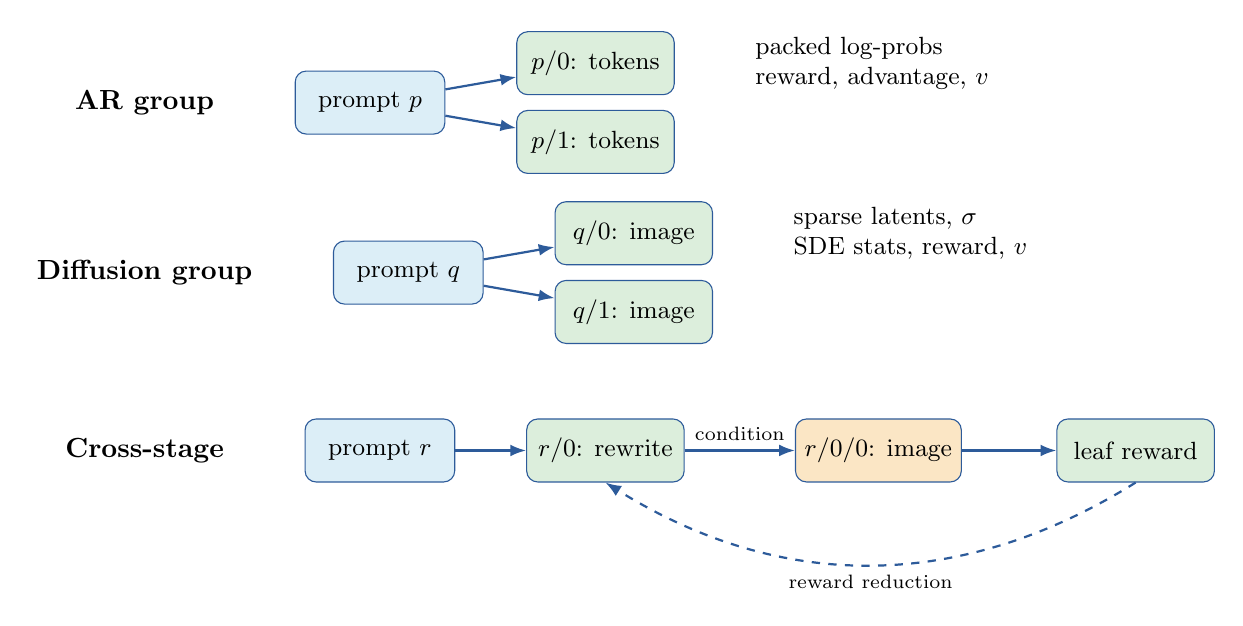
\begin{tikzpicture}[
  node distance=5mm and 9mm,
  every node/.style={font=\small},
  root/.style={draw=unirlblue,rounded corners,fill=unirlcyan,minimum width=19mm,minimum height=8mm},
  gen/.style={draw=unirlblue,rounded corners,fill=unirlgreen,minimum width=20mm,minimum height=8mm},
  obs/.style={draw=unirlblue,rounded corners,fill=unirlorange,minimum width=20mm,minimum height=8mm},
  arr/.style={-{Latex[length=2mm]},thick,draw=unirlblue}
]
\node[font=\bfseries] (arlabel) {AR group};
\node[root,right=of arlabel] (arp) {prompt $p$};
\node[gen,right=of arp,yshift=5mm] (ar0) {$p/0$: tokens};
\node[gen,right=of arp,yshift=-5mm] (ar1) {$p/1$: tokens};
\draw[arr] (arp) -- (ar0);
\draw[arr] (arp) -- (ar1);
\node[right=of ar0,align=left] {packed log-probs\\reward, advantage, $v$};

\node[font=\bfseries,below=16mm of arlabel] (dlabel) {Diffusion group};
\node[root,right=of dlabel] (dp) {prompt $q$};
\node[gen,right=of dp,yshift=5mm] (d0) {$q/0$: image};
\node[gen,right=of dp,yshift=-5mm] (d1) {$q/1$: image};
\draw[arr] (dp) -- (d0);
\draw[arr] (dp) -- (d1);
\node[right=of d0,align=left] {sparse latents, $\sigma$\\SDE stats, reward, $v$};

\node[font=\bfseries,below=17mm of dlabel] (clabel) {Cross-stage};
\node[root,right=of clabel] (cp) {prompt $r$};
\node[gen,right=of cp] (rewrite) {$r/0$: rewrite};
\node[obs,right=14mm of rewrite] (image) {$r/0/0$: image};
\node[gen,right=12mm of image] (credit) {leaf reward};
\draw[arr] (cp) -- (rewrite);
\draw[arr] (rewrite) -- node[above,font=\scriptsize]{condition} (image);
\draw[arr] (image) -- (credit);
\draw[arr,dashed,bend left=32] (credit.south) to node[below,font=\scriptsize]{reward reduction} (rewrite.south);
\end{tikzpicture}}
\caption{Three trajectory shapes represented by the same ordered-part IR. A generated part retains decoded values and the optimization segment required to replay its policy. The policy version $v$ is attached to generated frontiers. The cross-stage path illustrates available ancestry; E4 freezes the rewrite model and trains only diffusion.}
\label{fig:trajectory-ir}
\end{figure}

\subsection{Values, conditions, and segments are separate layers}

\system distinguishes three kinds of leaves that are often conflated.

\paragraph{Primitives.}
Primitives are decoded or externally supplied values: text, images, videos, audio waveforms, and media references.
Image pixels and variable-duration video/audio values use packed representations with per-example shapes or cumulative offsets.
They are suitable for reward functions, visualization, and subsequent turns, but need not be the tensors replayed by the trainable model.

\paragraph{Conditions.}
Conditions are model-facing encodings, such as text embeddings or image latents.
They allow rollout adapters and train-side stages to agree on typed inputs without prescribing one tokenizer, text encoder, or multimodal fusion architecture.

\paragraph{Segments.}
Segments retain optimization-facing state.
\texttt{TextSegment} stores variable-length packed token fields.
\texttt{LatentSegment} stores latent snapshots at selected indices, a shared sigma schedule, and optional SDE log probabilities or transition means.
The sparse index map is important: a diffusion algorithm can replay only selected transitions instead of materializing an entire denoising path for every loss.

The distinction makes decoded payload lifetime independent of replay lifetime.
After reward logging, trainers may drop large decoded media while retaining conditions, segments, reward, and credit for training.

\subsection{A field algebra defines structural batching}

Every structured batch field declares a composition rule: concatenated, packed variable-length, shared, or reduced by maximum, minimum, sum, or mean.
These annotations drive concat, split, selection, repetition, and device movement recursively.
They also define how a distributed method reconstructs its return value.
For example, a DP-scattered rollout receives a tree-complete shard and returns parts that are merged position-wise; a broadcast lifecycle method returns one replicated control result.

This is a stronger contract than requiring each role to hand-author tensor slicing.
It also creates a measurable cost: recursive structural operations and reference bookkeeping must be benchmarked in Section~\ref{sec:rq3} rather than assumed free.

\subsection{Rollout engines implement one transformation}

Every rollout engine fills a request and returns a trajectory:
\begin{equation}
F_{\theta,e}: \mathcal{T}_{\mathrm{request}} \longrightarrow \mathcal{T}_{\mathrm{filled}},
\label{eq:engine}
\end{equation}
where $e$ identifies a train-side or external generation runtime.
The base contract also exposes lifecycle and policy-publication operations, but it does not standardize the engine's internal serving API.

The current source contains four useful forms of Equation~\ref{eq:engine}.
The train-side adapter invokes the model pipeline directly under evaluation mode.
Dedicated SGLang and vLLM-Omni adapters translate typed trajectory inputs to their native requests and rebuild typed responses.
A composed engine serially fills multiple generated parts, for example an AR rewrite followed by diffusion generation.
An agentic engine repeatedly appends policy turns and environment observations.
The claim is therefore about a common boundary, not one universal generation kernel.

\subsection{The algorithm boundary preserves specialized replay}

A train stack owns microbatch planning, gradient accumulation, global loss normalization, gradient clipping, optimizer steps, and per-update aggregation.
An algorithm object owns the stage-specific map
\begin{equation}
(C,Z,A;\theta) \longmapsto \mathcal{L}\quad\text{and backward}.
\label{eq:algorithm}
\end{equation}
Before repeated optimizer updates, the stack can freeze an old-policy anchor at the same microbatch geometry used for training.
AR objectives replay token log probabilities; diffusion objectives replay selected transitions and may compare rollout statistics, a pre-update replay, or a reference model.
Supervised and forward-process objectives explicitly opt out of advantages.

This division is deliberately not advertised as algorithmic novelty.
GRPO follows the group-relative formulation introduced for language reasoning~\citep{shao2024deepseekmath}; PPO follows proximal policy optimization~\citep{schulman2017ppo}; diffusion objectives build on prior diffusion-RL methods~\citep{black2023ddpo,liu2025flowgrpo,xue2025dancegrpo,zheng2025diffusionnft}.
The systems question is whether these objectives can consume the same trajectory and execution contracts without hiding their different sufficient statistics.

\section{From a Program to a Distributed Execution}
\label{sec:execution}

Figure~\ref{fig:architecture} separates the feedback program from the mechanisms that execute it.

\begin{figure}[H]
\centering
\resizebox{\textwidth}{!}{%
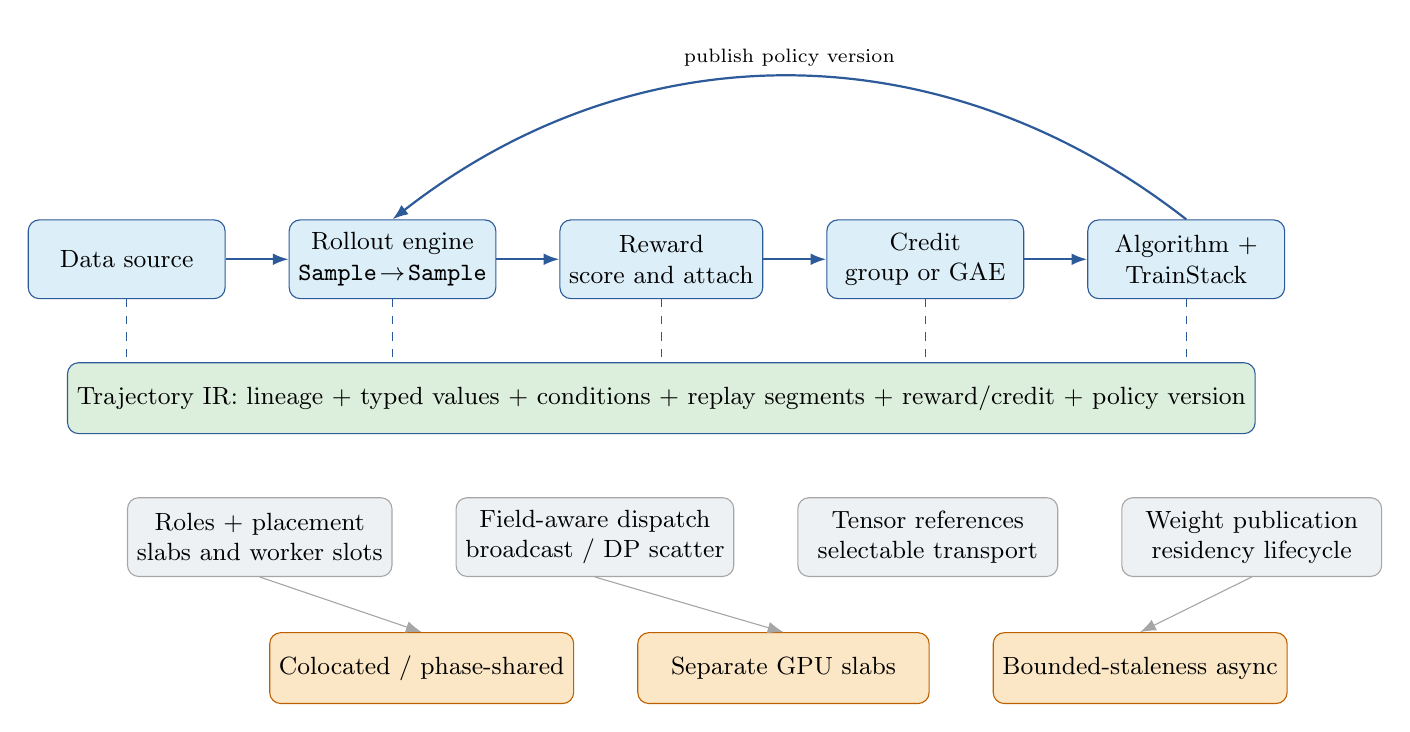
\begin{tikzpicture}[
  every node/.style={font=\small},
  role/.style={draw=unirlblue,rounded corners,fill=unirlcyan,minimum width=25mm,minimum height=10mm,align=center},
  ir/.style={draw=unirlblue,rounded corners,fill=unirlgreen,minimum height=9mm,align=center},
  mech/.style={draw=gray!70,rounded corners,fill=unirlgray,minimum width=33mm,minimum height=10mm,align=center},
  topo/.style={draw=orange!75!black,rounded corners,fill=unirlorange,minimum width=37mm,minimum height=9mm,align=center},
  arr/.style={-{Latex[length=2mm]},thick,draw=unirlblue}
]
\node[role] (data) {Data source};
\node[role,right=8mm of data] (rollout) {Rollout engine\\$\sample\!\rightarrow\!\sample$};
\node[role,right=8mm of rollout] (reward) {Reward\\score and attach};
\node[role,right=8mm of reward] (credit) {Credit\\group or GAE};
\node[role,right=8mm of credit] (train) {Algorithm +\\TrainStack};
\draw[arr] (data) -- (rollout);
\draw[arr] (rollout) -- (reward);
\draw[arr] (reward) -- (credit);
\draw[arr] (credit) -- (train);
\draw[arr,bend right=38] (train.north) to node[above,font=\scriptsize]{publish policy version} (rollout.north);

\node[ir,below=8mm of reward,minimum width=132mm] (irbar) {Trajectory IR: lineage $+$ typed values $+$ conditions $+$ replay segments $+$ reward/credit $+$ policy version};
\draw[dashed,draw=unirlblue] (data.south) -- (data.south |- irbar.north);
\draw[dashed,draw=unirlblue] (rollout.south) -- (rollout.south |- irbar.north);
\draw[dashed,draw=unirlblue] (reward.south) -- (reward.south |- irbar.north);
\draw[dashed,draw=unirlblue] (credit.south) -- (credit.south |- irbar.north);
\draw[dashed,draw=unirlblue] (train.south) -- (train.south |- irbar.north);

\node[mech,below=8mm of irbar,xshift=-51mm] (place) {Roles + placement\\slabs and worker slots};
\node[mech,right=8mm of place] (dispatch) {Field-aware dispatch\\broadcast / DP scatter};
\node[mech,right=8mm of dispatch] (transport) {Tensor references\\selectable transport};
\node[mech,right=8mm of transport] (lifecycle) {Weight publication\\residency lifecycle};

\node[topo,below=7mm of dispatch,xshift=-22mm] (coloc) {Colocated / phase-shared};
\node[topo,right=8mm of coloc] (separate) {Separate GPU slabs};
\node[topo,right=8mm of separate] (async) {Bounded-staleness async};
\draw[-{Latex[length=2mm]},draw=gray!70] (place.south) -- (coloc.north);
\draw[-{Latex[length=2mm]},draw=gray!70] (dispatch.south) -- (separate.north);
\draw[-{Latex[length=2mm]},draw=gray!70] (lifecycle.south) -- (async.north);
\end{tikzpicture}}
\caption{Source-derived UniRL architecture. The top row is the feedback program; the green bar is its stable data boundary. The lower rows map logical roles to communication and resource policies. Not every topology is valid for every engine; startup validation rejects unsupported combinations.}
\label{fig:architecture}
\end{figure}

\subsection{Logical roles, device slabs, and worker slots}

A \texttt{DevicePool} creates one Ray worker per GPU initially and reserves one strict-packed placement group per node.
A placement scope selects a fraction of currently available devices.
Roles created inside a scope either share its worker slot---enabling local sibling access and memory time-sharing---or receive isolated slots on the same devices.
Disjoint top-level scopes form separate training, rollout, or reward slabs.

A role is a regular Python object derived from \texttt{Remote}.
The handle constructs one role replica on each selected worker and derives data-, tensor-, pipeline-, sequence-, and expert-parallel rank metadata from the role configuration.
Method decorators state argument dispatch and return collection.
The trainer is consequently a single-controller program, while each method may invoke multi-controller distributed training or serving inside a role.
This resembles HybridFlow's separation between orchestration and distributed computation~\citep{sheng2024hybridflow}; UniRL's paper claim centers instead on carrying the same typed lineage through heterogeneous generative stages.

\subsection{Tensor references decouple structure from movement}

Before an RPC, dense tensor leaves may be \emph{dehydrated} into \texttt{TensorRef}s.
A reference is an ordered list of half-open row spans over opaque handles, plus shape, dtype, and device metadata.
Selection and contiguous slicing construct new span views without moving tensor data.
At a destination, hydration resolves all referenced spans in a batch and reconstructs the original nested object.

The transport interface has a deliberately small contract: store tensors, resolve handles, identify references, and optionally localize references for destination workers.
The audited source provides (i) a colocated per-worker store, (ii) a per-GPU store with IPC and NCCL transfers, and (iii) a TransferQueue path backed by simple storage or Mooncake-compatible storage.
Mooncake itself was proposed for disaggregated serving~\citep{qin2024mooncake}; here its storage interface is a transport option rather than a claimed UniRL invention.

The driver can therefore manipulate trajectory structure and metadata without materializing all GPU tensors.
Whether this reduces memory and transfer cost in practice is RQ3, not an assumption.

\subsection{Phase lifecycles and policy publication}
\label{sec:lifecycle}

Training and generation often hold different copies or formats of a policy.
UniRL exposes their interaction as an ordered lifecycle:
\begin{enumerate}
  \item wake the rollout engine sufficiently to receive weights;
  \item publish parameters if the cadence requires it;
  \item optionally offload colocated training state;
  \item generate and stamp the frontier with the engine's policy version;
  \item sleep the engine when the selected residency policy requires it;
  \item restore training state before replay and optimization.
\end{enumerate}

The concrete order varies by engine capabilities.
For example, staged wake can receive weights before mapping the rest of an AR engine, and a train-side engine reads live model objects without a separate publication role.
Separate slabs use an explicit one-time handshake.
Weight-sync implementations cover LoRA tensor paths and several full-weight paths, including tensor serialization, CUDA IPC, NCCL, and checkpoint rendezvous.
The base engine can also receive per-track updates for composed models.

The source rejects combinations whose lifecycle has not been validated, such as a train-side rollout on a physically separate slab or selected EMA/offload combinations.
This fail-closed policy is important because a partially awakened engine or silently stale adapter can produce plausible but invalid training data.
Section~\ref{sec:evaluation} therefore includes replay-consistency and failure-injection checks alongside throughput.

\subsection{Synchronous execution}

The synchronous AR trainer performs rollout, reward, credit assignment, replay/update, optional evaluation, and checkpointing in order.
The diffusion trainer can accumulate multiple rollouts into one optimizer window and can place reward on the train slab or a third slab.
In both cases, topology affects resource ownership and residency but not the trajectory boundary.
This makes a controlled topology experiment possible: hold model, prompts, group size, reward, number of replayed steps or tokens, and optimizer updates constant while changing only engine or placement.

\subsection{Bounded-staleness execution}
\label{sec:async}

Asynchrony changes correctness conditions, not just control flow.
UniRL's asynchronous AR and diffusion trainers share one manager.
A background dispatcher fills every engine slot up to a configured per-worker capacity.
Completed trajectories are grouped by root; only complete groups enter the ready buffer.
Every generated part must carry an output policy version $v_o$.

Let $v_t$ be the current optimizer-update version and $u$ the number of optimizer updates performed per consumed rollout batch.
The manager exposes lag in update units,
\begin{equation}
\ell = v_t-v_o \leq u b,
\end{equation}
where $b$ is the configured staleness allowance in rollout-batch units; the filter rejects work beyond that budget.
Before publishing version $v_t$, it pauses admission, drains or suspends work, completes any started or batch-aligning prefix, checks that no publication splits a training batch across behavior versions, publishes weights, updates the rollout version, and then resubmits eligible pristine carry.
Evaluation and checkpointing require a fully empty manager.

This discipline differs from claiming fully asynchronous optimization.
Weight publication remains a barrier, and the current asynchronous diffusion path deliberately limits in-flight batch structure more tightly than the AR path.
The evaluation must report the actual lag histogram, dropped work, and barrier time; a nominal ``async'' label is insufficient.

\section{Instantiations of the Common Contracts}
\label{sec:instantiations}

The following paths show which information crosses the common boundary and which computations remain specialized.

\subsection{Autoregressive reasoning}

An input part carries prompt text and metadata.
Forking by group size creates generated shells with sibling IDs.
An AR engine fills packed token segments and decoded text, a reward role attaches scalar or component rewards, and the part computes group-normalized credit or token-level generalized advantage estimates.
The train stack replays the same segment and applies the selected objective.
Optional token-length balancing permutes complete samples before DP sharding, preserving sibling identifiers and precomputed credit.

\subsection{Diffusion and flow generation}

A diffusion request forks prompts and records sampling parameters, a sigma schedule, selected SDE indices, and an initial-noise recipe.
The engine returns decoded media plus a latent segment whose sparse trajectory fields are sufficient for the selected update.
FlowGRPO-style objectives replay recorded steps and compare new transition log probabilities against a frozen rollout or replay anchor~\citep{liu2025flowgrpo}.
Forward-process objectives such as DiffusionNFT use clean generated samples rather than the same reverse-trajectory likelihood path~\citep{zheng2025diffusionnft}.
The common train stack handles microbatching and optimizer state; the algorithm remains responsible for these incompatible estimators.

\subsection{Cross-stage and environment-interacting trajectories}

In a prompt-enhancement path, one root produces one or more AR rewrites, and every rewrite produces one or more images.
The image reward is attached to the leaf; when the rewrite stage trains, parent-major reduction supplies its feedback.
The primary E4 case freezes that stage and uses ancestry to select the diffusion advantage groups.
In a tool-interacting path, the policy emits an action-like text part, the environment appends an observation part, and the process repeats until termination or suspension.
Both workflows need ancestry to survive rollout scheduling and sharding; flattening them into unrelated rows would require rebuilding that correspondence out of band.

E4 checks these groups against an explicit ID-based reference and then studies the two grouping objectives in training.

\section{Evaluation Design and Prespecified Protocol}
\label{sec:evaluation}

We organize evaluation around four research questions.
Each reported run must archive the resolved configuration, commit and dirty diff, model and dataset revisions, environment manifest, raw logs, structured metrics, parser version, and evaluation outputs.
Primary comparisons use the same hardware one framework at a time.
The operational commands, run-directory schema, and failure-routing rules are frozen in
\codepath{GPU\_HANDOFF\_README.md}; the stricter evidence-admission contract is in
\codepath{EXPERIMENT\_RUNBOOK.md}.

\begin{table}[H]
\caption{Prespecified experiment-to-claim map. E0 is a gate, not a result; P0 rows are required to close the paper's primary trajectory-centric claim.}
\label{tab:experiment-map}
\centering
\scriptsize
\begin{tabularx}{\textwidth}{@{}llL{0.31\textwidth}Y@{}}
\toprule
ID & Priority & Controlled study & Paper evidence \\
\midrule
E0 & P0 gate & Environment, semantic parity, replay/publication, checkpoint, and instrumentation checks & Evaluation validity and Appendix~\ref{app:correctness} \\
E1 & P0 & Qwen3-4B-Base GRPO on DAPO-Math, three seeds & RQ1 AR validity; matched reference pending \\
E2 & P0 & SD3.5-Medium FlowGRPO, three seeds per system and external image evaluation & RQ1 long-run reference and collapse guards \\
E3 & P0 & Shape-matched native UniRL--VeRL-Omni SD3.5 recipes on eight GPUs & RQ2 throughput, resources, and phase cost \\
E4 & P0 & Frozen-Qwen prompt enhancement with original-prompt versus rewrite-local grouping & RQ3 lineage and enablement result \\
E5 & P0 minimum & IR/transport costs plus a matched UniRL topology pair & RQ3 abstraction and execution cost \\
E6 & P1 & Matched synchronous/asynchronous Qwen3 sweep & RQ4 lag--quality--time trade-off \\
\bottomrule
\end{tabularx}
\end{table}

The order is E0, then E1--E4 and the minimum E5 topology/cost slice; E6 and broader E5 scaling/transport backends follow.
If compute is limited, we complete primary E0--E5 before adding more models, algorithms, or scaling points: without E4 the paper would not directly test lineage, and without the minimum E5 slice it would not bound the cost of that abstraction.

\paragraph{Environment fields intentionally left open.}
The experimental design fixes semantic work before the allocation is known, but does not guess hardware facts.
The GPU model, node count, GPUs per node, NVLink/PCIe/InfiniBand topology, CPU, driver and compatibility libraries, exact local model snapshot hashes, input/evaluator hashes, AR baseline commit, and released run IDs are currently ``--'' and will be populated directly from admitted manifests.

\subsection{RQ1: Does UniRL reproduce credible training behavior?}
\label{sec:rq1}

The first question is scientific rather than purely operational.
A successful run must improve over its frozen base on prespecified external endpoints without diagnostic collapse.
This establishes learning validity. Reproducing another implementation additionally requires a full-budget reference with disclosed semantic differences; a 30-step speed run cannot supply that evidence.
E2 therefore includes a long-run VeRL-Omni reference, while the adapted AR reference remains a separate prerequisite for an AR reproduction claim.

\paragraph{AR workload.}
E1 trains Qwen3-4B-Base~\citep{yang2025qwen3} with full-parameter GRPO on DAPO-Math-17k~\citep{yu2025dapo}.
The data name does not imply use of the DAPO optimizer; we fix the population-standard-deviation group estimator implemented in the audited recipe.
Each rollout contains 64 prompts with eight samples (512 trajectories), uses SGLang TP=1 with thinking enabled, temperature/top-$p$ 1.0, top-$k$ disabled, and at most 8192 new tokens.
The learner uses group-standard-deviation normalization, symmetric clipping at 0.2, \texttt{seq-mean-token-mean} aggregation, four updates per rollout, a 10,240-token microplanner, AdamW learning rate $10^{-6}$ and weight decay 0.01, and full-weight publication every rollout.
We prespecify 800 rollouts on 32 total GPUs, internal AIME evaluation every ten rollouts, full checkpoints every 200 rollouts, and seed IDs 11, 22, and 33 applied to data order and the SGLang server RNG.
Frozen base and checkpoints 200/400/600/800 are evaluated on MATH-500 (500 problems, avg@4) and AIME 2024/2025 (30 problems each, avg@16) using the registry's fixed decoding and \texttt{math\_verify} grader.
The UniRL run and the selected current reference must align prompts, chat template, verifier, maximum generation length, group size, effective batch, clipping, KL treatment, optimizer updates, and evaluation decoding.
The public veRL Qwen3 FSDP example is only a scaffold because its stock model variant, data, group size, response budget, and KL/objective settings differ; the AR reference row remains blank until a pinned adapted launcher passes a resolved-config parity audit.
The final 800-rollout checkpoint is primary. Internal evaluation uses AIME 2024/2025, so an AIME-selected best checkpoint is reported only as validation-selected and cannot establish an untouched AIME test result.
MATH-500 is the primary external AR endpoint, with a training/evaluation overlap audit required before interpretation; the fixed-budget AIME curves are secondary diagnostics.
We report every seed, final-checkpoint curves, and 95\% confidence intervals; avg@$k$ denotes mean accuracy across $k$ sampled answers, not pass@$k$.

\paragraph{Diffusion workload.}
E2 fixes SD3.5-Medium~\citep{sd35medium2024} and the UniRL FlowGRPO setting used by E3: 48 prompts with 16 images (768 samples) per rollout, $384\times384$ training resolution, ten denoising steps, three SDE steps in the first half, $\eta=0.8$, guidance 1, and distinct initial noise.
PickScore~\citep{kirstain2023pickapic} supplies the training reward; advantages subtract each prompt-group mean and divide by the batch-wide reward standard deviation.
LoRA rank/alpha is 32/64 on eight matched attention projections; the learner uses two updates, microbatch eight, learning rate and weight decay $10^{-4}$, clip $10^{-5}$, and publication every rollout.
We prespecify 300 rollouts on one eight-GPU node with seed IDs 11, 22, and 33.
The same budget and seed IDs apply to the pinned VeRL-Omni reference; checkpoint export and estimator parity are audited before admission.
The stock pair differs in SDE strategy, step selection, and potentially normalization/anchor semantics, so it currently defines a related-recipe comparison. At least one full-budget E1 or E2 reference must pass mathematical and work parity before the paper claims reference-implementation reproduction; otherwise that claim remains unestablished.
Frozen base and every 50-rollout checkpoint use a shared diffusers evaluation pipeline. The primary image endpoint is PartiPrompts HPSv3~\citep{ma2025hpsv3}; ImageReward~\citep{xu2023imagereward} and compositional scores provide complementary checks.
These are held-fixed automatic judges distinct from the optimized PickScore model, not independent human studies.

\paragraph{Image evaluation identity.}
The registry key \texttt{image/geneval2} points to UniRL's \texttt{synthetic/test.jsonl} and a local Qwen3-VL-8B Soft-TIFA-style scorer.
We name this the \emph{synthetic compositional set}; it is not an official GenEval~2 result~\citep{kamath2025geneval2} without a separate data-and-scorer parity audit.
Both image endpoints use $512\times512$, 40 steps, guidance 1, one image per prompt, and an evaluation seed of 42 shared across training seeds and checkpoints.
The synthetic endpoint additionally fixes its explicit linear sigma grid, prompt-hashed seeds, and 256-token text-encoder limit; the preference endpoint fixes the pinned pipeline schedule and index-based seeds.
Dataset sizes, revisions, overlap counts, and scorer hashes remain open manifest fields.

The diversity guard is within-prompt mean pairwise LPIPS~\citep{zhang2018lpips} (AlexNet features), computed over 16 images per PartiPrompts prompt at the same evaluation setting, with identical image seeds for base and checkpoint.
We average all 120 pair distances per prompt, then report the relative change in the mean across prompts and a paired prompt-bootstrap interval.
A greater than 10\% relative decrease is a study-specific investigation trigger; it is not a literature-established quality threshold. A near-zero base makes this relative criterion undefined and requires the absolute change to be reported.
This guard diagnoses collapse and is not itself a perceptual-quality metric.

\begin{table}[H]
\caption{Planned single-stage training-validity matrix. Dashes are deliberately not numerical placeholders.}
\label{tab:rq1}
\centering
\small
\begin{tabularx}{\textwidth}{@{}lXllll@{}}
\toprule
ID & Workload / external endpoint & Base & Reference/control & UniRL & Seeds \\
\midrule
E1 & Qwen3-4B-Base GRPO; MATH-500/AIME & \multicolumn{3}{c}{\emph{in progress --- seed 11 at rollout 470/800; primary endpoint is the rollout-800 checkpoint}} & 0/3 \\
\midrule
\multicolumn{6}{@{}l}{E2 --- SD3.5-M FlowGRPO, 1{,}632 prompts at $K{=}16$, 26{,}112 images per preference row, 19/19 rows scored, 0 errors} \\
E2a & HPSv3, held-out preference (primary endpoint) & 1.2024 & -- & \textbf{9.8126} & 3 \\
E2b & ImageReward, held-out preference & -- & -- & $\Delta\,{+}1.3932$ & 3 \\
E2c & PickScore, the optimized objective & -- & -- & $\Delta\,{+}0.0970$ & 3 \\
E2d & Composition, synthetic compositional (vqascore) & 0.1011 & -- & \textbf{0.1552} & 3 \\
E2e & Diversity, within-prompt LPIPS guard & -- & -- & $\Delta\,{-}24.79\%$ & 3 \\
\bottomrule
\end{tabularx}
\par\vspace{1mm}
The UniRL column gives the endpoint level where a base level is recorded, and a change ($\Delta$) where only the paired difference is; the two are not interchangeable and are marked rather than mixed.
Per-seed values, the statistical unit being the seed: HPSv3 gain $8.579/8.713/8.538$, mean $+8.6102$, 95\% $t$ interval $[8.383,\,8.837]$; composition $+54.5/+50.4/+55.5\%$, mean $+53.5\%$, $[46.8,\,60.1]$; diversity $-23.95/-25.19/-25.22\%$, mean $-24.79\%$, $[-26.59,\,-22.99]$.
At three seeds the $t$ interval carries $2$ degrees of freedom and is wide by construction; the per-seed values, not the interval, are the reportable evidence.
\emph{The diversity guard fired on all three seeds}, and the narrowing is already present at rollout 50 ($-15.69/-14.08/-12.91\%$), so truncating the budget does not avoid it.
PickScore, the optimized objective, rises monotonically at all six checkpoints while both frozen judges flatten after checkpoint 150.
\par\vspace{1mm}
\paperTODO{Still open: the E2-R VeRL-Omni reference column --- three seeds are trained and their exports audited (15/15 consecutive pairs, native $=$ export bit-identical), but no held-out evaluation was run because the estimator mismatch between the stacks is unresolved. Also outstanding: exact checkpoint revisions and released run IDs. The E1 row is absent rather than pending.}
\end{table}

\subsection{RQ2: What is end-to-end system performance?}
\label{sec:rq2}

E3 is the primary performance comparison: UniRL versus VeRL-Omni commit \texttt{01c87ee5} for the E2 SD3.5 shape-matched work unit on one reserved eight-GPU node~\citep{verlomni2026}.
Both sides use 48 prompts, 16 samples, $384\times384$ output, ten denoising steps, three early-window SDE steps, two optimizer updates, microbatch eight, LoRA 32/64 on the same projections, learning rate/weight decay $10^{-4}$, clip $10^{-5}$, and PickScore.
We run three process-level repetitions per configuration, 30 steps each, remove exactly the first five timing observations, and retain at least 20 observations per repetition.
Systems run one at a time on the same hosts with matched cache and clock policy; each repetition block randomizes their order.
We report a backend-aligned SDPA-class row and separately each system's preregistered best valid backend.
The stock UniRL recipe uses \texttt{FlowSDEStrategy} and three sampled early indices; the VeRL-Omni launcher requests \texttt{cps} and an early three-step window.
These may change the transition distribution and likelihood, not merely kernel implementation. Normalization, anchors, actual replay work, and reward-service GPU placement also require an audit.
Until a semantically aligned pair is established, E3 is labeled a \emph{shape-matched native-recipe comparison}; attention-backend matching alone does not make it an equivalent-algorithm framework comparison.
Its speed ratio cannot be attributed solely to framework overhead.

An E1 AR comparison is secondary and remains blocked until the adapted veRL launcher matches model, data, prompt/chat template, verifier, generation budget, effective batch, estimator, token packing, optimizer work, publication, and evaluation.
If semantic parity cannot be achieved, the row is omitted rather than replaced by a nearby recipe.

Metrics include median, mean, and p90 iteration time after a prespecified warmup; samples/s and samples/GPU-hour; per-phase time for generation, reward, credit, anchor/replay, backward/optimizer, weight publication, wake/sleep, and barriers; peak allocated and reserved GPU memory by role; CPU memory; and utilization.
Strong and weak scaling use fixed global and fixed per-GPU work, respectively, after the primary single-node pair is complete.
The 30-step E3 protocol does not support a time-to-quality claim; E2's long-run comparison supplies quality context, and E6 prespecifies a threshold-based study.

\begin{table}[H]
\caption{Systems result schema. Every cell will be derived from archived raw artifacts.}
\label{tab:rq2}
\centering
\small
\begin{tabularx}{\textwidth}{@{}lXrrrr@{}}
\toprule
System & Configuration & s/iter & samples/s & samples/GPU-h & peak GiB \\
\midrule
UniRL & Native flow / SDPA-class & \textbf{64.22} & 11.96 & \textbf{5381} & 75.4 \\
VeRL-Omni & Native CPS / SDPA & 111.33 & 6.90 & 3104 & 28.4 \\
UniRL & preregistered best valid & 64.22 & 11.96 & 5381 & 75.4 \\
VeRL-Omni & FA3 best valid & 112.26 & 6.84 & 3079 & 28.4 \\
\bottomrule
\end{tabularx}
\par\vspace{1mm}
Median seconds per iteration, aggregated as the median of three replicate medians, after removing the first five timing observations and retaining at least 20 per replicate.
Replicate spread: UniRL $0.76$\,s ($1.18\%$), SDPA $1.11$\,s ($0.99\%$), FA3 $1.99$\,s ($1.78\%$).
\textbf{UniRL is $1.73\times$ faster than the SDPA row and $1.75\times$ faster than FA3}; the two VeRL-Omni rows are statistically indistinguishable, so \emph{FA3 versus SDPA is a null}.
UniRL's preregistered best valid backend is its SDPA-class configuration, so those rows coincide.
\par\vspace{1mm}
Two qualifications belong with the headline rather than below it.
\emph{The median is the reported unit because the mean is not stable on one arm}: the VeRL-Omni arm takes a $>3\sigma$ upward excursion roughly once per run (worst retained step $119.76$\,s, $\approx 1.08\times$ its median) and the UniRL arm never does, with mean $\approx$ median throughout --- so a reader preferring means would see a \emph{larger} UniRL advantage.
\emph{The pair is not parameter-matched}: bare versus prefix-qualified LoRA targets give 243 against 191 modules ($23.9$M versus $18.8$M, $1.27\times$), and the parameter-matched ratio is $1.70\times$, which is the conservative figure.
\par\vspace{1mm}
\paperTODO{Still open: strong and weak scaling, deferred by design until the single-node pair closed; and the per-phase breakdown panel. Peak GiB is the maximum across the three replicates of each configuration. Failed and retried iterations are accounted for in the archived per-step series.}
\end{table}

\subsection{RQ3: What does the trajectory abstraction cost and enable?}
\label{sec:rq3}

RQ3 first tests the semantic capability that motivates the IR, then measures its cost.
E4 uses the executable frozen-Qwen3-0.6B rewrite $\rightarrow$ SD3.5 path: eight original prompts, four rewrites per prompt, and eight images per rewrite, or 256 image descendants per rollout; only diffusion trains.
This is a separate recipe from E2: $512\times512$, ten steps, one sampled SDE index among 0--8, $\eta=0.7$, LoRA 16/32, learning rate $3\times10^{-4}$, weight decay zero, clip $10^{-4}$, replay anchor, two updates, and microbatch one.
The primary condition computes group-relative advantages across all 32 descendants of one original prompt, while \texttt{diffusion\_group\_scope=rewrite} groups the eight images under each rewrite.
Both conditions must serialize redacted root/part/parent IDs, shapes, reward/advantage, replay indices, group labels, and output versions.
Invalid lineage remains an E0 fail-fast test rather than an intentionally corrupted quality baseline.

For image $x_{p,j,k}$, the two group keys are $g_{\rm root}=p$ and $g_{\rm rewrite}=(p,j)$.
First, on identical recorded rewards and replay tensors, an ID-joined flat-row reference must reproduce UniRL's group memberships, advantages, and learner inputs for each key, including after root-shard round trips.
The subsequent 300-rollout, three-seed training comparison changes the normalization population (32 versus eight images); its quality difference is therefore an objective effect, not a causal measurement of the IR's superiority.

This control establishes that retained ancestry selects a real optimization grouping; it does not by itself prove better task quality.
The current PickScore request is conditioned by the rewritten text, so a claim about preserving the user's original intent additionally requires lineage-keyed evaluation of every image against its root prompt.
We therefore report both rewrite-conditioned training reward and frozen HPSv3/ImageReward evaluations joined to each root prompt.
Evaluation generates held-out images at $512\times512$, 40 steps, and guidance 1 with the base and every 50-rollout diffusion checkpoint, using one fixed manifest of four frozen rewrites per root and eight image seeds per rewrite for both conditions.
Worker/adapter RNG initialization, deterministic trainside-AR sampling, real trace dumping, and this held-out generation/evaluation path are E0 prerequisites for a multi-seed E4 result.
If the two correct groupings tie, the experiment still establishes semantic expressiveness but not a quality benefit.

\paragraph{E4 result: the semantic control passes, the quality comparison is a null.}
The ID-joined flat-row reference reproduces UniRL's group memberships, advantages, and learner inputs for both keys, \textbf{24/24 checks in both scopes} --- including root-shard split$\rightarrow$concat and roots shuffled and reconstructed by ID, with the float32 reduction bit-exact against the ID join.
\emph{This is the result that establishes retained ancestry selects a real optimization grouping}, and it stands independently of what follows.
The 300-rollout, three-seed training comparison between root-scope and rewrite-scope grouping is a \textbf{null}: the seeds disagree in sign.
A paired bootstrap over 64 roots on a single seed gave root-conditioned HPSv3 $+0.387$ $[+0.085,\,+0.706]$, which three seeds do not sustain; the binding constraint is seed count rather than rewrite quality.
Consistent with the prespecified interpretation, this negative result is retained rather than repaired by hyperparameter search.

One disclosure is required for the measured arm to be interpretable: at the audited commit the frozen rewriter has \emph{no} \texttt{pe} block, so both frozen-LLM variants drop \texttt{pe\_instruction}/\texttt{pe\_marker} and raw chat replies become SD3 conditioning.
Of 256 rewrites, 71\% carry chat markers, 73\% exceed CLIP's 77-token window, and 0 contain the marker.
The correction was written but deliberately not applied, so the measured rows remain attributable to a single configuration.
Because the grouping comparison is a null, this is a property of the arm that was measured rather than a defect that changed a reported effect.

We then measure recursive IR operations and tensor transport separately from model compute.
Microbenchmarks vary root count, branch factor, number and size of tensor leaves, ragged token/media lengths, and part depth.
They report split/concat/select latency, reference metadata bytes, dense bytes avoided at the driver, same-GPU and cross-GPU transfer time, cross-node time when available, and correctness hashes after reassembly.

E5 compares the colocated store, per-GPU store, and TransferQueue path where the hardware supports them.
At the audited commit the full GPU transport harness is not yet checked in, so implementation and review of that harness is an explicit prerequisite rather than an implied result.
We compare whole-tree sharding against the explicit ID-joined flat-row reference on the same recorded payloads and with the same transport.
This paired representation slice holds model work, device placement, values, grouping, and replay inputs fixed; driver RSS, bytes moved, operation time, and fraction of iteration cost measure the price of preserving structure.
Semantic errors are caught in E0 and are never timed as valid work.

The minimum topology slice reuses E3's colocated SD3.5 UniRL row and adds the same work with \codepath{sd3\_vllmomni\_lora\_separate.yaml}: four GPUs train and four generate while the total eight-GPU allocation remains fixed.

This pair measures two deployment regimes, not a pure transport primitive---training parallelism, residency, and local versus remote LoRA publication change together and are reported in the phase breakdown.
Broader same-/cross-GPU and cross-node backend measurements remain E5 extensions.

\paragraph{E5-T result: separating the slabs costs $2.277\times$ per iteration.}
Three replicates, all exiting zero, with 54/54 archived checksums verifying.
Colocated T0 is $64.223$\,s per iteration ($63.526/64.223/64.284$ across replicates, spread $0.758$\,s or $1.18\%$, 5{,}381 samples/GPU-hour); the separate $4{+}4$ topology T1 is $146.244$\,s on the same eight GPUs at the same effective work.
\emph{Consistent with the preceding paragraph, the ratio may not be attributed to \texttt{layout} alone} --- the per-phase breakdown is the deliverable and the multiplier is a summary of it.
The sentence to lead with is narrower and more informative: \textbf{under separate topology UniRL is slower than VeRL-Omni colocated} ($146.244$\,s against $111.33$\,s), so the allocation/residency cost of splitting the slabs exceeds the framework gap it was measured against.
\emph{E5-R is not reported: the checked-in harness does not measure the paired representation slice described above}, and whether to build a corrected harness or narrow RQ3 to the topology result is an open decision rather than pending work.
We inventory which bundle/stage/adapter code the existing E4 path uses and which trainer, scheduler, transport, and credit modules it shares. This documents reuse; reduced integration effort would require a separate held-out implementation study.

\paragraph{Preliminary executable evidence.}
We ran a source-importing regression harness against a clean UniRL checkout at
\texttt{f5d7104}; it does not mock the trajectory classes.
All ten checks passed: cross-stage lineage construction, exact tree split/concat,
whole-tree select/slice, leaf-to-root reward propagation and group advantages,
rejection of malformed lineage and primitive modality/batch violations, variable-length packed-text
round trips, and lazy \texttt{TensorRef} selection/materialization including bounds
checking.
Table~\ref{tab:cpu-ir} reports a deliberately narrow timing slice from the same run.
The synthetic workload has four AR children per root, one observation per AR child,
two diffusion children per observation, and a four-value image payload per leaf.

\begin{table}[H]
\caption{Preliminary single-process CPU trajectory-IR timings (microseconds).
Python 3.12.14 and PyTorch 2.11.0; one thread; ten warm-up and 100 measured repetitions.
These are regression measurements, not distributed or GPU throughput.}
\label{tab:cpu-ir}
\centering
\scriptsize
\input{artifacts/trajectory_ir/cpu_f5d7104_macos_arm64/summary_table.tex}
\end{table}

The current \texttt{Sample.select} path forms tree-complete root shards before
gathering them, so its cost grows with the full input tree rather than only the
selected rows. Strided \texttt{TensorRef} selection creates many metadata spans
while contiguous selection coalesces them; no dense tensor is copied until
materialization. These observations motivate, but do not replace, the planned
GPU transport and end-to-end ablations. The manifest, 100 per-cell raw trials,
structured check outcomes, generated table rows, and SHA-256 checksums are archived
under \codepath{artifacts/trajectory\_ir/cpu\_f5d7104\_macos\_arm64/}.

\subsection{RQ4: When is bounded-staleness execution useful?}
\label{sec:rq4}

E6 compares E1-derived runs with the same 32-GPU allocation, 64-by-eight rollout work unit, four optimizer updates, reward, evaluator, and 800-rollout budget; disaggregated points fix half the GPUs for training and half for rollout and keep \texttt{per\_worker\_inflight=14}.
The colocated synchronous point S0 and disaggregated zero-overlap point D0 reveal the allocation/residency cost of separating the slabs; D0 and A1 then test the onset of allowed overlap within the same disaggregated trainer and topology. This changes both in-flight capacity and lag allowance, so it is not a single-knob causal effect.
After a capacity pilot, the remaining primary grid fixes \texttt{max\_inflight=2} and varies publication interval and allowed lag as shown in Table~\ref{tab:async-sweep}.
Only after the primary grid may in-flight capacity one and four be added at one fixed publication/lag point.
Natural generation variance is stratified by prompt and response length; any synthetic-delay study is labeled as a secondary stress test.
Results include generation-latency distributions, engine occupancy, trainer idle fraction, publication/barrier time, completed and discarded samples, realized lag histograms, reward/eval versus optimizer update, and reward/eval versus wall time.
The key plot is a Pareto frontier of time-to-quality and realized policy lag.

\begin{table}[H]
\caption{Prespecified E6 primary points. Each uses seed IDs 11, 22, and 33. Configured lag is in consumed rollout batches; one batch performs four optimizer updates.}
\label{tab:async-sweep}
\centering
\small
\begin{tabularx}{\textwidth}{@{}lL{0.18\textwidth}rrrY@{}}
\toprule
Point & Trainer / topology & In-flight & Publish interval & Max lag (batches) & Purpose \\
\midrule
S0 & sync / colocated & -- & 1 & 0 & Total-resource reference \\
D0 & async / disaggregated & 1 & 1 & 0 & Same-topology no-overlap control \\
A1 & async / disaggregated & 2 & 1 & 1 & Onset of allowed overlap \\
A2 & async / disaggregated & 2 & 1 & 2 & Isolate lag allowance \\
A3 & async / disaggregated & 2 & 2 & 2 & Isolate publication cadence \\
A4 & async / disaggregated & 2 & 2 & 4 & Aggressive bounded point \\
\bottomrule
\end{tabularx}
\end{table}

\paragraph{Pilot result: no threshold was registered, and the budget is past its useful point.}
The capacity pilot ran all six points at one seed with evaluation off, giving per-rollout rates of $82.34$ (S0), $103.07$ (D0), $56.48$ (A1), $55.19$ (A2), $33.47$ (A3) and $39.54$\,s (A4, pooled over two replicates).
These are planning inputs, not results: one seed each, and A4 is the only pooled point.

The separate \texttt{Q\_TARGET} pilot then \textbf{failed its own preregistered rule, so no threshold is registered}.
Scoring D0 checkpoints offline on MATH-500 avg@4 gives $0.7980$ at rollout 150 (two independent scorings, $0.7960$ and $0.8000$) against $0.7730$ at rollout 300.
The rule required rollout 300 to exceed rollout 150; it is \textbf{lower by $0.0250$}, a paired $t$ of $-2.66$ over 500 prompts ($p \approx 0.008$) and $1.68\times$ the evaluation-noise half-width registered in advance to judge it.
The internal AIME evaluation agrees in direction on a different benchmark, sampler and dataset ($0.0927 \rightarrow 0.0802$).
\emph{Training reward rose $0.10 \rightarrow 0.43$ over the same span while held-out accuracy fell}, which is reward overfitting; at one point and two checkpoints the evidence carries a direction rather than a located turning point, so the supported claim is that held-out quality turns over somewhere between rollouts 150 and 300.
The same shape appears on the diffusion side, where PickScore rises monotonically while both frozen judges flatten (Section~\ref{sec:rq1}).

Consequently \emph{no time-to-quality figure is reported for this pilot}: $\Delta T = \epsilon / Q'(t)$ requires a positive quality-per-second, and $Q'$ is negative on this segment, so the conversion is undefined rather than large.

\paragraph{The evaluation-noise floor, and a limit it places on every checkpoint comparison.}
Two independent scorings of the \emph{same} checkpoint differ by $0.40$ aggregate accuracy points, but \textbf{agree on only 380 of 500 prompts}: 120 prompts changed between 1 and 4 of their 4 samples.
The paired standard error is $0.00759$, so $\pm 1.5$ accuracy points at 95\%.
Plumbing checks pass --- identical prompt identifier set, exactly four completions per prompt in both runs --- so this is a floor rather than an invalidation, and \texttt{-{}-random-seed} does not pin per-request sampling.
\textbf{It follows that no per-prompt, per-subset or per-difficulty claim from a single scoring is reliable}; aggregate stability here comes from averaging, not from sampling repeatability.

\paragraph{A controlled pair does not yet exist in the stock recipes.}
At the audited commit, the nominal Qwen3 GRPO sync and async example files differ in five fields that affect either the estimator or learner execution (Table~\ref{tab:sync-async-preflight}).
Consequently, measurements from those files without overrides are inadmissible as evidence about asynchrony.
The GPU study will first choose one value for every controlled field, apply explicit overrides, archive both fully resolved Hydra configurations, and produce a field-by-field parity report.
Only topology, concurrency, publication interval, and allowed policy lag may then vary.

\begin{table}[H]
\caption{Mandatory preflight corrections for the stock Qwen3 GRPO sync/async pair at commit \texttt{f5d7104}. These are source/config observations, not results.}
\label{tab:sync-async-preflight}
\centering
\scriptsize
\begin{tabularx}{\textwidth}{@{}L{0.29\textwidth}YYL{0.30\textwidth}@{}}
\toprule
Controlled field & Sync stock & Async stock & Required action \\
\midrule
\texttt{normalize\_adv\_by\_std} & \texttt{true} & \texttt{false} & Match the advantage estimator. \\
High clipping bound & unset & \texttt{0.28} & Match symmetric/asymmetric clipping. \\
Loss aggregation & sequence mean, then token mean & sequence mean, token sum normalized & Match sequence-length weighting. \\
Attention implementation & \texttt{flex\_attention} & default & Match for backend-aligned rows. \\
Microplanner & token budget, 10,240 & default count planner & Match packing and learner work. \\
\bottomrule
\end{tabularx}
\end{table}

\paragraph{Measurement readiness.}
The current structured logger supplies six coarse phases, rollout diagnostics, GPU memory counters, and output/train/published versions with realized lag.
Its \texttt{perf/step\_time\_s} field is insufficient as an end-to-end clock: the async trainer logs it before the outer loop's quiescence, publication, evaluation, and checkpoint work.
E3/E6 therefore require driver-level monotonic timestamps spanning complete iterations and the full run; phase timers are reconciled against that clock rather than summed across overlapping roles.
Before RQ2 and RQ4, instrumentation must separate credit, replay/anchor, backward, optimizer, checkpoint, and publication-barrier time, and must emit complete per-step series for buffer occupancy and admitted, carried, suspended, rejected, discarded, retried, and completed work.
GPU utilization and power must be collected by an external monitor synchronized to the run clock.
Missing structured fields may not be reconstructed from isolated console messages or dashboard screenshots.

\paragraph{Predeclared interpretation and escalation.}
Expected directions are hypotheses rather than results.
For E1, the primary external MATH-500 endpoint should improve from the base without collapse in length, truncation, group variance, ratio, or clipping diagnostics.
For E2, held-out HPSv3 should improve with the optimized PickScore while compositional, ImageReward, and diversity checks diagnose regressions.
For E3, competitive throughput must survive complete end-to-end and failure accounting.
For E4, lineage/group membership must be exact, while a quality advantage for original-prompt grouping must be judged against root prompts and remains optional evidence rather than an invariant.
For E6, moderate lag should reduce idle time and may improve time-to-quality, whereas aggressive lag may increase rejection or harm quality.
Configuration, logging, parity, lineage, version, checkpoint, and replay/publication faults are engineering failures to diagnose and rerun under a new ID.
Changing the optimizer, reward, estimator, formal budget, model/task, evaluator, aligned-baseline definition, or central claim requires a research decision and a newly registered experiment.
Stable negative results after correctness passes are retained; they are not repaired by silent hyperparameter search.

\paperTODO{The formal E6 grid has not run. Two items gate it: the six buffer counters above are unwritten, and \texttt{rejected} --- the mechanism bounded staleness acts through --- is constructed each step and never counted, which makes the async points inadmissible as specified. The evaluation-path stall that previously prevented S0 from running was diagnosed and fixed upstream, and the fix is validated at 32 devices, so the S0-vs-D0 allocation/residency contrast is no longer deferred; its runs have not been made. Result panels for learning curves, phase breakdown, scaling, utilization, and the throughput--policy-lag Pareto frontier follow the grid.}

\subsection{Fairness and statistical protocol}

Effective work is matched before wall-clock time: prompts, samples per prompt, decoded resolution or maximum tokens, rollout steps, replayed steps/tokens, microbatching semantics, and optimizer updates.
Primary full-system metrics count all allocated training, rollout, and reward resources on both sides. Reward placement and concurrency must be disclosed; a reward-excluded number is supplementary and carries a separate service-cost report.
We prespecify warmup removal, use at least 20 steady-state iterations for throughput summaries, and report the full distribution rather than a single minimum.
Training summaries use the seed as the statistical unit, show every seed, and report the mean with a 95\% $t$ interval; bootstrap intervals over prompts or images are labeled separately and never substituted for seed uncertainty.
Systems summaries show all three process-level repetitions and the pooled per-step distribution after the fixed five-observation warm-up; uncertainty of a speed ratio uses repetitions, not correlated steps, as its independent units.
The final checkpoint and named primary endpoint are fixed in advance; the auxiliary metrics diagnose failure modes and are not alternative endpoints chosen after seeing results.
Time-to-quality in E6 uses MATH-500 and a threshold recorded before the formal grid, based only on a separate pilot. We report the first observed checkpoint crossing, bracket it by adjacent evaluation times, and censor runs that never cross.
Elapsed time spans initialization, training, publication, checkpointing, and evaluation; steady-state throughput is reported separately.
All published cells require complete scoring or an explicit missingness analysis; silently averaging only successful evaluator responses is inadmissible.

\section{Related Work}
\label{sec:related}

\paragraph{LLM post-training systems.}
HybridFlow/veRL combines single- and multi-controller execution and introduces hierarchical APIs for mapping RLHF dataflows to devices~\citep{sheng2024hybridflow}.
OpenRLHF uses Ray, vLLM, and DeepSpeed to schedule the models in an RLHF workflow~\citep{hu2024openrlhf}.
ROLL emphasizes a single-controller abstraction, parallel workers, sample lifecycle scheduling, and flexible device mapping~\citep{wang2025roll}.
NeMo-RL provides scalable training and generation backends and multimodal model support~\citep{nemorl2025}.
UniRL shares their concern for composable orchestration; its intended distinction is the lineage- and modality-aware trajectory boundary across AR, diffusion, and cross-stage generation.
That distinction must be established by RQ3 rather than a feature table.

\paragraph{Asynchronous post-training.}
AReaL fully decouples generation and training and controls staleness to improve language-reasoning throughput~\citep{fu2025areal}.
Relax uses service-level separation, a TransferQueue data bus, and configurable staleness for omni-modal post-training~\citep{zhang2026relax}.
slime supports persistent asynchronous rollout generation around a training/rollout/data-buffer loop~\citep{slime2025}.
These systems make asynchrony an execution design space, not a UniRL novelty claim.
UniRL implements a version-stamped group and publication-boundary discipline shared by AR and diffusion paths; RQ4 tests whether that realization is useful, without claiming a new asynchronous RL algorithm.

\paragraph{Multimodal and diffusion post-training systems.}
VeRL-Omni extends veRL toward diffusion, unified, and omni-modality models and integrates vLLM-Omni rollout~\citep{verlomni2026}.
Relax is explicitly omni-native~\citep{zhang2026relax}.
Accordingly, ``supporting image, video, or audio'' cannot be the paper's contribution.
The comparison instead asks how ancestry, typed replay state, and movement compose at the trajectory boundary. E4 tests one concrete workflow; a universal claim of easier integration is outside its evidence scope.

\paragraph{Diffusion RL algorithms.}
DDPO casts denoising as a multi-step decision process~\citep{black2023ddpo}.
Flow-GRPO converts flow sampling to an SDE and applies group-relative optimization~\citep{liu2025flowgrpo}; DanceGRPO generalizes related ideas across visual generation tasks~\citep{xue2025dancegrpo}; DiffusionNFT instead optimizes a forward-process objective from reward-ranked generations~\citep{zheng2025diffusionnft}.
UniRL implements several algorithm families but does not claim their mathematical ideas.
Its algorithm interface keeps their incompatible replay state explicit while reusing scheduling and training mechanics.

\section{Limitations and Open Evidence}
\label{sec:limitations}

\paragraph{Integration is not automatic.}
Each new architecture still needs a bundle, stages, conditions, and adapters for the selected rollout runtime.
A common trajectory type does not eliminate tokenizer, scheduler, latent-layout, LoRA-target, or serving-version incompatibilities.
The current ordered-frontier operations also assume compatible depths and parent-contiguous groups; arbitrary ragged forests, shared-field equality, and adversarial row order are not uniformly validated by the container itself.

\paragraph{Topology is configured, not optimized.}
Placement scopes make resource choices explicit but do not search for the best split.
The best topology depends on model memory, reward cost, rollout variance, interconnect, and publication size.

\paragraph{Asynchronous execution is bounded and partially specialized.}
Publication is a barrier, and current AR and diffusion paths impose different admissible in-flight structure.
Fault isolation is limited by the shared Ray runtime and role lifecycle; the system does not yet claim service-level recovery comparable to dedicated service architectures.

\paragraph{The empirical case is incomplete.}
At the audited commit, raw logs sufficient to verify existing benchmark prose were absent from the checkout.
Therefore this draft makes no end-to-end throughput, scaling, memory, convergence, or final-quality claim.
Sections~\ref{sec:rq1}--\ref{sec:rq4} define the evidence required to remove this limitation.

\section{Conclusion}

\system treats post-training as a trajectory program whose semantic object survives changes in generative family and execution topology.
Lineage, typed modality values, replay segments, reward, credit, and policy version live in one IR; rollout, reward, training, transport, and publication are logical roles mapped separately to resources.
This design is most valuable if it passes two empirical tests: credible learning behavior across representative AR and diffusion workloads, and competitive end-to-end execution without weakening semantic parity.
Those tests are necessary but not sufficient for the paper's trajectory-centric thesis: a real composed run must also demonstrate lineage-defined credit/grouping, and the measured IR/topology costs must bound the price of preserving that structure.
The final paper will be complete only when artifact-backed evaluation establishes this full claim chain; bounded-staleness remains a conditional operating-region result rather than a prerequisite for every deployment.

\section*{Reproducibility statement}

The source characterization in this draft refers to UniRL commit
{\small\texttt{f5d710406b215bb7a0b387fdd37e4d4778b92338}} (2026-08-20).
The manuscript repository records the claim-to-evidence plan in \texttt{PAPER\_PLAN.md}.
The cluster-ready execution protocol, configuration-parity gates, metric inventory,
and immutable run-directory contract are specified in
\texttt{EXPERIMENT\_RUNBOOK.md}; the command-oriented transition to a fresh GPU-side
agent is in \texttt{GPU\_HANDOFF\_README.md}. Both documents intentionally contain
no results.
The preliminary RQ3 evidence is regenerated by
\codepath{experiments/trajectory\_ir/run\_cpu\_evidence.py}; its manifest pins the
source state, command, environment, workload, warm-up, repetitions, and timer.
\paperTODO{Before release, add the public artifact DOI/URL and author metadata, then archive manifests and regeneration scripts for every remaining result and figure.}

\bibliographystyle{tmlr}
\bibliography{main}

\appendix

\section{Claim-to-source audit}
\label{app:source-audit}

Table~\ref{tab:source-audit} records the executable source used to support mechanism descriptions.
It does not prove performance or successful execution for every configuration.

\begin{table}[H]
\caption{Primary code evidence at commit \texttt{f5d7104}.}
\label{tab:source-audit}
\centering
\scriptsize
\begin{tabularx}{\textwidth}{@{}L{0.20\textwidth}Y@{}}
\toprule
Mechanism & Primary source symbols \\
\midrule
Trajectory IR & \codepath{unirl/types/sample.py}: \texttt{Part}, \texttt{Sample}; \codepath{unirl/types/primitives.py}; \codepath{unirl/types/segments/} \\
Batch algebra & \codepath{unirl/distributed/tensor/batch.py}: \texttt{FieldKind}, \texttt{Batch} \\
Tensor references & \codepath{unirl/distributed/tensor/ref.py}: \texttt{TensorSpan}, \texttt{TensorRef}; \codepath{transport.py}: \texttt{TensorTransport} \\
Roles and placement & \codepath{unirl/distributed/group/device\_pool.py}, \codepath{placement.py}, \codepath{handle.py}, \codepath{dispatch.py} \\
Rollout boundary & \codepath{unirl/rollout/engine/base.py}: \texttt{BaseRolloutEngine}; concrete engines under \codepath{unirl/rollout/engine/} \\
Training boundary & \codepath{unirl/algorithms/base.py}: \texttt{StageAlgorithm}; \codepath{unirl/train/stack/base.py}: \texttt{TrainStack} \\
Sync trainers & \codepath{unirl/trainer/ar.py}: \texttt{ARTrainer}; \codepath{unirl/trainer/diffusion.py}: \texttt{DiffusionTrainer} \\
Async scheduler & \codepath{unirl/trainer/async\_rollout.py}; \codepath{unirl/rollout/manager/} \\
Weight publication & \codepath{unirl/distributed/weight\_sync/}; engine-specific receivers under \codepath{unirl/rollout/engine/} \\
Instrumentation & \codepath{unirl/utils/profiling.py}, \codepath{memory\_monitor.py}, \codepath{wandb\_logger.py} \\
\bottomrule
\end{tabularx}
\end{table}

\section{Required run artifact schema}
\label{app:artifacts}

Every result row must resolve to a run directory containing:
\begin{itemize}
  \item source and baseline commit hashes, submodule hashes, and dirty patches;
  \item the launch command and fully resolved configuration;
  \item model, reward, dataset, and tokenizer revisions or content hashes;
  \item GPU model/count, node/interconnect description, driver, CUDA, PyTorch, generation-engine, and training-backend versions;
  \item raw stdout/stderr, per-step structured timing, memory and utilization traces, checkpoint metadata, and evaluation outputs;
  \item seed, warmup exclusion rule, failure/retry accounting, and statistical aggregation script.
\end{itemize}

For training runs, serialized trace samples must redact private data while retaining lineage IDs, shapes, dtypes, policy versions, reward components, and segment index metadata.
For system baselines, an alignment manifest must explain every nonidentical setting and whether it changes effective work.

\clearpage
\section{Correctness status and remaining checks}
\label{app:correctness}

\paragraph{Executed locally.}
The preliminary RQ3 harness performs ten fail-fast checks on the audited source:
lineage-valid cross-stage construction; exact split/concat; tree-complete select and
slice; mean reward propagation plus group-normalized advantages; rejection of bad
lineage, modality keys, and primitive batch sizes; packed variable-length text
select/concat; and lazy tensor-reference selection, materialization, identity, and
bounds behavior. The structured outcomes and data-sensitive SHA-256 round-trip hash
are stored with the run artifacts.

\paragraph{Required before performance interpretation.}
The following system-level checks remain prerequisites for all applicable RQs:
\begin{enumerate}
  \item \textbf{Rollout--replay parity:} before the first update, compare engine-emitted and train-side replay log probabilities or transition statistics under stated numerical tolerances.
  \item \textbf{Publication parity:} repeat the parity check after each LoRA or full-weight publication path used in an experiment.
  \item \textbf{Batch-version integrity:} verify that an optimizer batch never mixes behavior versions when the configured algorithm assumes one version.
  \item \textbf{Boundary integrity:} checkpoint and evaluation begin only after the async manager is empty; resume restores the optimizer version and republishes it before new rollout.
  \item \textbf{Work accounting:} compare generated tokens or pixels, denoising and replay steps, scored samples, and committed optimizer updates across systems.
  \item \textbf{Structural preconditions:} validate unique root IDs, equal frontier depth, parent-major grouping, shared-field equality, and version provenance before merging or propagating credit; check against an ID-joined reference.
\end{enumerate}

\end{document}
